\section{Sistemas autónomos. Plano de fases}

Ya hemos pasado por un tema de sistemas lineales donde aprendimos a resolver cosas de la forma \[ \begin{cases}x'= a_{11}x + a_{12}y \\ y'=a_{21}x + a_{22}y \end{cases} \]. Ahora veremos sistemas de la forma \[ \begin{cases} x'(t) = F(x,y) \\ y'(t) = G(x,y) \end{cases} \]. Trabajaremos en dimensión dos para dibujar de forma mucho más precisa los sistemas, pero la teoría será genérica.

El detalle importante de estos sistemas es que en la parte derecha no aparece la variable $t$, lo que nos da un resultado básico: si $X(t) = (x(t), y(t))$ es solución, entonces también lo es $X_h(t) = (x(t+h), y(t+h))\; ∀h∈ℝ$. Es decir, las soluciones serán \textbf{invariantes por traslación}. Obtendremos la solución concreta al fijar el dato inicial.

En vista de este resultado, normalmente interpretaremos las soluciones $(x(t), y(t)) = σ(t)$, una curva parametrizada que dibujaremos en el plano.

Consideremos de nuevo el sistema masa resorte, con la ecuación $x'' +kx = 0$. Si lo escribimos como sistema, tenemos \[ \begin{cases} x' = y \\ x' = -kx \end{cases} \], que nos daba una solución explícita 

\begin{align*}
x(t) = A\cos \sqrt{k}t + B \sin \sqrt{k} t \\
y(t) = B\sqrt{k}\cos \sqrt{k} t - A \sqrt{k}\sin \sqrt{k} t
\end{align*}

Supongamos que no hemos sabido resolver el sistema y no hemos encontrado la solución. Simplemente mirando el sistema deberíamos apreciar un punto importante: $x(t) = 0,\;y(t) = 0$ es una solución. Si lo pintamos en el plano de fases, la trayectoria sería un único punto en el origen. Se trata de una solución estacionaria o punto de equilibrio.

\begin{definition}\name{Punto}[de equilibrio]
En general, diremos que $(a,b)$ es un punto de equilibrio si y sólo si $F(a,b) = G(a,b) = 0$.
\end{definition}

Esto nos da un primer camino a estudiar: la \textbf{estabilidad}. 

El segundo problema a estudiar sería el comprobar si hay \textbf{trayectorias cerradas}. Es decir, queremos encontrar soluciones periódicas. Encontraremos un problema similar al de la estabilidad: ¿qué pasa cuando cogemos una solución que pasa por un punto cercano a una trayectoria cerrada? ¿Sigue estando cerrada o se abre? 

Volviendo al problema del sistema masa-resorte: si sabemos que buscamos una curva parametrizada, ¿podemos escribirlo como conjunto de nivel? No siempre es posible pero a veces funciona. En el caso de que efectivamente podamos eescribir la solución como conjunto de nivel $E(x,y) = C$, tendríamos que

\begin{gather*}
\pd{E}{x}  x' + \pd{E}{y}y' = 0 \\
\pd{E}{x} y + \pd{E}{y} (-kx) = 0
\end{gather*}
o, dicho de otra forma, buscamos que $\grad E \perp (y,-kx)$. En este caso, $\grad E$ sería paralelo a $(kx,y)$ y obtendríamos las trayectorias dadas por la ecuación

\[ \frac{kx^2}{2} + \frac{y^2}{2} = C 
\]
lo que, en el plano de fases nos daría algo como la imagen \ref{img:FasesMasaResorte}. Ahora bien, ese dibujo no estaría completo: nos faltaría determinar el sentido en el que recorremos las curvas, que lo obtendríamos viendo la derivada.

\begin{figure}[hbtp]
\centering
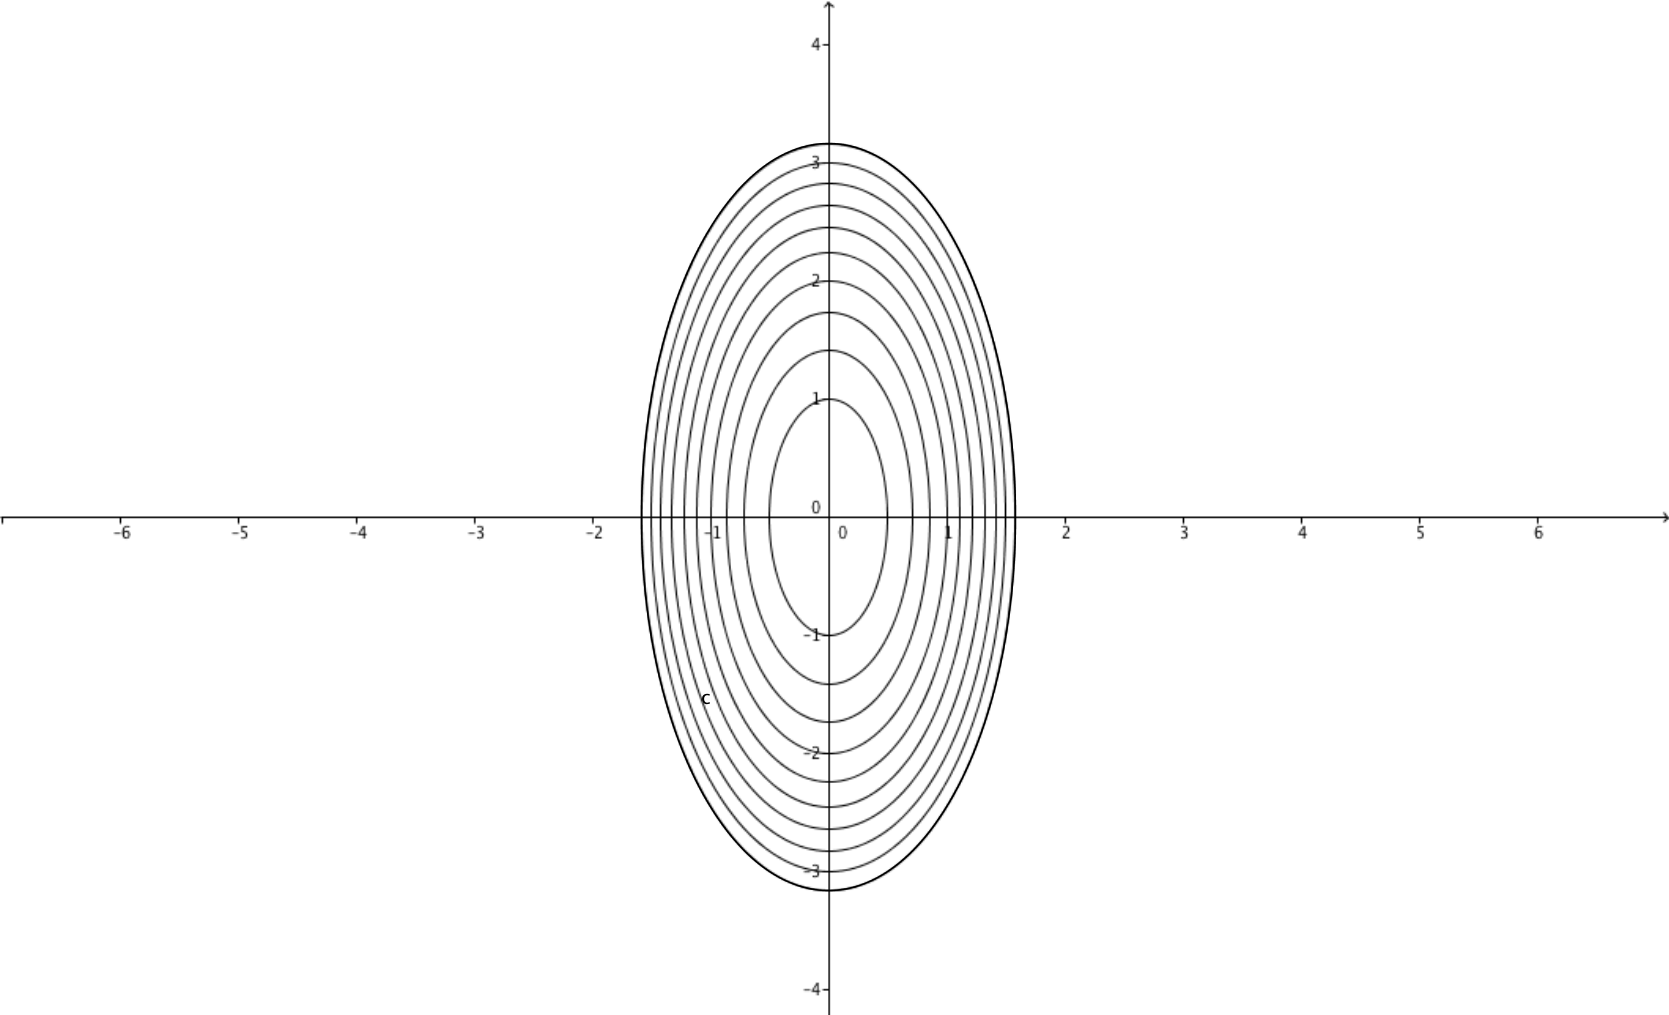
\includegraphics[width=0.8\textwidth]{img/PlanoFasesMasaResorte.png}
\caption{Plano de fases para el sistema masa-resorte}
\label{img:FasesMasaResorte}
\end{figure}

Si fuésemos físicos, veríamos que la $x$ sería la posición y $y$ la velocidad, representando en un diagrama ambas variables. Pero como no lo somos, nos la repantinfla bastante.


Si aplicamos esta misma idea a sistemas generales del estilo, \[ \begin{cases} x' = F(x,y) \\ y' = G(x,y) \end{cases} \], llegamos a la siguiente definición:

\begin{definition}\name{Integral}[ primera] Decimos que $E(x,y) ∈ C^1$ es una \textbf{integral primera} del sistema si y sólo si dado $(x(t),y(t))$ solución, entonces $E(x(t),y(t)) = C\;∀t$.
\end{definition} 

Esta integral primera no siempre existe. Pero, si por ejemplo tenemos un sistema \[ \begin{cases} x' = \pd{H}{y}(x,y) \\ y' = -\pd{H}{x}(x,y) \end{cases} \] la integral primera es inmediata: $H(x,y) = C$. Los sistemas con este tipo de estructura se llaman \textbf{sistemas hamiltonianos}\index{Sistema!hamiltoniano}.

En el caso general, si tenemos una integral primera $E(x,y) = C$, entonces

\[ 0 = \pd{E}{x}x' + \pd{E}{y} y' = \pd{E}{x}F + \pd{E}{y} G 
\] 
lo que nos dice que buscamos $\grad E \perp (F,G)$ o, lo que es lo mismo, $\grad E \parallel (-G,F)$. Esto nos llevaría a que si \[ -\pd{G}{y} = \pd{F}{x}\] entonces tenemos que $(-G,F) = \grad V$ para un potencial $V$, y entonces podremos tomar $E\equiv V$. Si no encuentras esto, podemos buscar un factor integrante\footnote{Y lloras. Mucho.}.

\begin{example}
\[\begin{cases}x' = y \\ y' = 1+x^2 \end{cases} \]

Buscamos una solución de la forma $E(x(t), y(t)) = C$ que cumple 

\[ \grad E \perp (y, 1+x^2) \implies \grad E (1+x^2,-y) \]

Necesitamos entonces poder escribir $(1+x^2,-y)$ como $\grad V$, el gradiente de un potencial. Para ello, tendría que cumplirse que 

\[ \pd{}{y}(1+x^2) = \pd{}{x}(-y) \]

Efectivamente, en este caso se cumple y existe $V$. Integrando:

\begin{gather*}
\pd{V}{x} = 1+x^2 \implies V = x + \frac{x^3}{3} + C(y) \\
-y \stackrel{?}{=} \pd{V}{y} = C'(y) \implies C(y) = \frac{-y^2}{2}
V(x,y) = x + \frac{x^3}{3} -\frac{y^2}{2}
\end{gather*}

Por lo tanto, las soluciones serán las dadas por las curvas $V(x(t), y(t)) = C$, dibujadas en la figura \ref{imgGranos}. Sólo faltaría el sentido en el que se recorren las curvas. Viendo las derivadas, vemos que $y'>0$ y que por lo tanto se recorren hacia arriba siempre, hacia la derecha cuando $y$ es positivo y hacia la izquierda en otro caso.

\end{example}

\begin{figure}
\centering
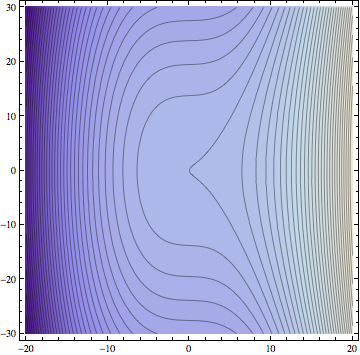
\includegraphics[width=0.5\textwidth]{img/Grano.png}
\caption{Conjuntos de nivel de la función $x + \frac{x^3}{3} -\frac{y^2}{2}$.}
\label{imgGranos}
\end{figure}

\begin{example}
\[ \begin{cases} x' = x(1+y) \\ y'=-y(1+x) \end{cases} \]

Buscamos de nuevo una posible función potencial. Hacemos las derivadas cruzadas:

\begin{gather*}
\pd{}{y} (y(1+x)) = 1+x \\
\pd{}{x} (x(1+y)) = 1+y
\end{gather*}

No existe un potencial que resuelva esta ecuación. Ahora bien, podemos buscar una función μ tal que $(μ(-G),μF)  = \grad V$. Derivamos de nuevo

\begin{align*}
\pd{}{y} (μy(1+x)) &\stackrel{?}{=} \pd{}{x} (μx(1+y)) \\
(1+x)\left(\pd{μ}{y} y + μ\right) &= (1+y)\left(\pd{μ}{x}  + μ\right)
\end{align*}

y si miramos, podremos encontrar un factor integrante.
\end{example}

\begin{example}[Tiburones en el océano]
Suponiendo que no hubiese predadores, el número de presas $x$ variaría linealmente con la tasa de supervivencia $a$, que depende de la diferencia entre mortalidad y natalidad. Es decir, \[ x' = ax \]. 

Con predadores, la ecuación se transformaría en \[ x' = a(y) x \], con $a$ dependiendo del número de predadores $y$. Si consideramos que $a(y)$ es una recta, por simplificar el modelo, la ecuación sería \[ x' = ax - bxy \].

Por otra parte, podemos considerar que la población de predadores crece con \[ y' = -cy + dxy \].

Transformando un poco las ecuaciones, llegamos al problema \[ \begin{cases} x' = x(a-by) \\ y' = y(-c+dx) \end{cases} \], que son las llamadas \textbf{ecuaciones de Volterra}. 

Este problema tiene puntos críticos $F=G=0$. Si $F=0$, podemos tener $x=0$, el caso obvio de que no hay ni presas ni predadores. El otro es que $y=\frac{a}{b}$, que nos da que para que $G=0$ debe de ser $x=\frac{c}{d}$, lo que nos daría un punto de equilibrio.

Si añadimos al sistema a los pescadores, con influencia ε ($a\to a + ε$, $c\to c+ ε$), el punto de equilibrio pasa a ser $\displaystyle \left(\frac{a-ε}{b}, \frac{c+ε}{d}\right)$, un punto más abajo y a la derecha. Es decir, se favorece la aparición de presas y la disminución de la proporción de predadores. En la segunda guerra mundial, al bajar la pesca el movimiento se invirtió y aumentó el porcentaje de tiburones.

Ahora bien, la naturaleza no siempre se mantiene en el punto de equilibrio, sino que hay oscilaciones. Veámoslo resolviendo el sistema. Buscamos una función $E(x,y) = C$. Las derivadas cruzadas no son iguales, por lo que hay que buscar un factor integrante $μ(x,y)$ tal que 

\[ \pd{}{y}(μ(x,y)(cy -dxy)) = \pd{}{x} (μ(x,y) (ax-bxy)) \]

Haciendo la cuenta, sale $μ(x,y) = \frac{1}{xy}$. La solución es entonces

\[ \grad V = \left(\frac{1}{xy}(xy-dxy),\frac{1}{xy}(ax-bxy)\right)= \left(\frac{c}{x}-d,\frac{a}{y}-b\right) 
\]
de donde podemos sacar \[ V(x,y) = a \log y - b y + c \log x - d x \]. 

Sólo nos interesa lo que pasa en el primer cuadrante (posiciones negativas no nos gustan). Lo que obtenemos son trayectorias cerradas alrededor de un punto de equilibrio (figura \ref{imgPoblaciones})
\end{example}

\begin{figure}[hbtp]
\centering
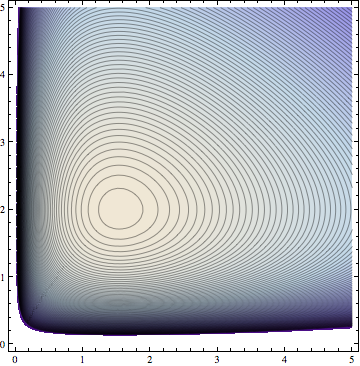
\includegraphics[width=0.5\textwidth]{img/Poblaciones.png}
\caption{Evolución de presas y depredadores.}
\label{imgPoblaciones}
\end{figure}

\begin{theorem}
Sea $(x_1(t), y_1(t))$ una solución tal que $(x_1(t),y_1(t)) ∈ γ\; ∀t$ donde γ es una curva en el plano de fases.

Sea $(x_2(t), y_2(t))$ otra solución y supongamos que existen $t_1, t_2 ∈ ℝ$ tales que  $(x_1(t_1), y_1(t_1)) = (x_2(t_2),x_2(t_2))$. Entonces $(x_2(t), y_2(t)) ⊆ γ$.

Dicho de otra forma, si dos curvas solución se cortan entonces son la misma.
\end{theorem}

\begin{proof}
Sean $(x_h(t),y_h(t)) = (x_1(t+h), y_1(t+h))$. Sabemos que si $(x_1,y_1)$ es solución y estamos en un sistema autónomo, entonces $(x_h, y_h)$ también es solución. En particular, para $h=t_1 - t_2$ tenemos que \[ (x_{t_2 - t_1}(t),y_{t_2 - t_1}(t)) = (x_1(t+t_1-t_2),y_1(t+t_1-t_2)) \].

En el punto $t=t_2$, nos queda \[ (x_{t_2 - t_1}(t_2),y_{t_2 - t_1}(t_2)) = (x_1(t_1),y_1(t_1)) \].

Tenemos dos soluciones del sistema que en el instante inicial pasan por el mismo punto. Aplicando el teorema de existencia y unicidad, tenemos que $(x_{t_2 - t_1},y_{t_2 - t_1})\equiv (x_2,y_2)$, que no es más que una traslación de la solución original $(x_1,y_1)$.
\end{proof}

\subsection{Clasificación de puntos críticos}

Partimos del sistema \[ \begin{cases} x' = ax + by \\ y' = cx + dy \end{cases} \] con $a,b,c,d∈ℝ$, que viene de una \textit{linealización} por Taylor de cualquier sistema.

¿Cuántos puntos críticos tenemos? Sabemos que siempre tenemos al menos el $(0,0)$ como punto crítico. Si además la matriz $\begin{pmatrix} a & b \\ c & d \end{pmatrix}$ tiene determinante cero, tendremos una recta de puntos críticos.

Para el análisis, empezaremos suponiendo que $(0,0)$ es un punto crítico aislado, es decir, con \[ \det \begin{pmatrix} a & b \\ c & d \end{pmatrix} ≠ 0 \]. 

Vamos a ir paso a paso distinguiendo los distintos casos que nos podemos encontrar al resolver este sistema.

\subsubsection{Sistemas con autovalores reales}

\paragraph{Caso 1.1: $0< λ_1 < λ_2$}. Con esta información, la solución general es 

\[ \begin{pmatrix} x(t) \\ y(t) \end{pmatrix} = A e^{λ_1t}\begin{pmatrix} u_1 \\ u_2\end{pmatrix} + B e^{λ_2t} \begin{pmatrix} v_1 \\ v_2 \end{pmatrix} \].

En esta ecuación está toda la información que tenemos que tener sobre el plano de fases. Tenemos varias opciones. 

Si $A = 0$, la solución es \[ B e^{λ_2t} \begin{pmatrix} v_1 \\ v_2 \end{pmatrix} \]. Es decir, que si $B>0$ tendremos una semirrecta en la dirección de $\vv$, y si es negativo una semirrecta en la dirección contraria. La solución sería análoga para $B=0$. Podemos ver en la figura \ref{imgABUnoCero} el esquema de las soluciones.

\begin{figure}[hbtp]
\centering
\begin{tikzpicture}
\draw[->] (-4,0) -- (4,0);
\draw[->] (0,-4) -- (0,4);

\draw[very thick, red!40!white, directed] (0,0) -- (2,4) node[right] {$A=0; B>0$};
\draw[very thick, red!80!black, directed] (0,0) -- (-2,-4) node[left] {$A=0; B<0$};

\draw[very thick, orange!40!white, directed] (0,0) -- (4,2) node[above] {$A>0; B=0$};
\draw[very thick, orange!80!black, directed] (0,0) -- (-4,-2) node[below] {$A<0; B=0$};


\draw[->,thick,red] (0,0) -- (0.7,1.4) node[left] {$\vv$};
\draw[->,thick,orange] (0,0) -- (1.4,0.7) node[above] {$\vu$};


\end{tikzpicture}
\caption{Posibles soluciones para $A=0$ ó $B=0$.}
\label{imgABUnoCero}
\end{figure}

¿Qué ocurre cuando ni $A$ ni $B$ son cero? La solución general es \[ \begin{pmatrix} x(t) \\ y(t) \end{pmatrix} = A e^{λ_1t}\vu + B e^{λ_2t} \vv \]. Podemos sacar factor común $e^{λ_1t}$ para tener

\[ \begin{pmatrix} x(t) \\ y(t) \end{pmatrix} = e^{λ_1t} \left(A\vu + Be^{(λ_2-λ_1)t} \vv\right) \].

Es decir, que cuando $t\to -∞$, $Be^{(λ_2-λ_1)t} \to 0$ y por lo tanto la trayectoria será tangente al vector $\vu$. Si lo que hacemos es sacar factor común $e^{λ_2}$, tenemos 

\[ \begin{pmatrix} x(t) \\ y(t) \end{pmatrix} = e^{λ_2t} \left( Ae^{(λ_1-λ_2)t}\vu + B \vv\right) \].

Así, cualquier trayectoria en este caso acabará siendo paralela al vector $\vv$. Las trayectorias salen del origen tangentes a $\vu$ y cuando $t$ crece tienden a ser paralelas a $\vv$. Este último vector es la dirección principal, ya que atrae a todas las trayectorias salvo a la recta $\vu$ (cuando $A=0$).

\begin{figure}[hbtp]
\centering
\begin{tikzpicture}
\draw[->] (-4,0) -- (4,0);
\draw[->] (0,-4) -- (0,4);


\foreach \x in {0.5,1,1.5,2,2.5} 
	\draw[very thin, blue,dense directed] (0,0) to [looseness=\x,out=30, in=60] ({2*\x - 2},-4);

\foreach \x in {0.25,0.5,0.75} 
	\draw[very thin, blue,dense directed] (0,0) to [looseness=\x,out=210, in=60] ({-2 - 4*\x},-4);

\foreach \x in {0.25,0.5,0.75} 
	\draw[very thin, blue,dense directed] (0,0) to [looseness=\x,out=30, in=240] ({4*\x + 2},4);
	
\foreach \x in {0.5,1,1.5,2,2.5} 
	\draw[very thin, blue,dense directed] (0,0) to [looseness=\x,out=210, in=240] ({2 -2*\x},4);
	

\draw[very thick, red!40!white, directed] (0,0) -- (2,4);
\draw[very thick, red!80!black, directed] (0,0) -- (-2,-4);
\draw[very thick, orange!40!white, directed] (0,0) -- (4,2);
\draw[very thick, orange!80!black, directed] (0,0) -- (-4,-2);

\draw[->,thick,red] (0,0) -- (0.7,1.4) node[left] {$\vv$};
\draw[->,thick,orange] (0,0) -- (1.4,0.7) node[above] {$\vu$};


\end{tikzpicture}
\caption{Posibles soluciones (en azul) para $A=0$ ó $B=0$ con ambos autovalores positivos.}
\label{imgABNoCero}
\end{figure}

\paragraph{Caso 1.2: $λ_1 < 0 < λ_2$}. La solución es la misma que antes, \[ \begin{pmatrix} x(t) \\ y(t) \end{pmatrix} = A e^{λ_1t}\vu + B e^{λ_2t} \vv \].

Cuando $A=0$, tenemos el mismo caso de antes. Ahora bien, cuando $B=0$, al ser el autovalor negativo las soluciones \textit{vienen} de infinito. Es decir, tenemos el caso de la figura \ref{imgAB_AVN_UnoCero}

\begin{figure}[hbtp]
\centering
\begin{tikzpicture}
\draw[->] (-4,0) -- (4,0);
\draw[->] (0,-4) -- (0,4);

\draw[very thick, red!40!white, directed] (0,0) -- (2,4) node[right] {$A=0; B>0$};
\draw[very thick, red!80!black, directed] (0,0) -- (-2,-4) node[left] {$A=0; B<0$};

\draw[very thick, orange!40!white, directed] (4,2) node[above] {$A>0; B=0$} -- (0,0);
\draw[very thick, orange!80!black, directed] (-4,-2) node[below] {$A<0; B=0$} -- (0,0);


\draw[->,thick,red] (0,0) -- (0.7,1.4) node[left] {$\vv$};
\draw[->,thick,orange] (0,0) -- (1.4,0.7) node[above] {$\vu$};


\end{tikzpicture}
\caption{Las dos posibles rectas solución para un sistema autónomo con un autovalor negativo y otro positivo, con $A=0$ ó $B=0$.}
\label{imgAB_AVN_UnoCero}
\end{figure}

Cuando $A,B≠0$, siguiendo el mismo procedimiento de factores comunes de antes, tenemos que tanto en $+∞$ como en $-∞$ explotan. Cuando $t\to -∞$, estamos \textit{lejos} y paralelos a $\vu$. Cuando $t\to + ∞$, la trayectoria también se irá lejos en la dirección de $\vv$, tal y como refleja la figura \ref{imgAB_AVN_NoCero}.

\begin{figure}[hbtp]
\centering
\begin{tikzpicture}[spy using outlines={circle, magnification=4, size=2cm, connect spies}]
\draw[->] (-4,0) -- (4,0);
\draw[->] (0,-4) -- (0,4);

\foreach \x in {1,2,3} 
	\draw[very thin, blue,dense directed] (4,{2.5 - 0.1*\x }) to [looseness=\x,out=210, in=240] ({2.5 - 0.1*\x},4);

\foreach \x in {0.5,1,1.5,2} 
	\draw[very thin, blue,dense directed] (4,{1.7 + 0.1*\x }) to [looseness=\x,out=210, in=60] ({-1.5 - 0.2*\x},-4);

\foreach \x in {1,2,3,4} 
	\draw[very thin, blue,dense directed] (-4,{-2.5 + 0.1*\x }) to [looseness=\x,out=30, in=60] ({-2.5 + 0.1*\x},-4);

\foreach \x in {0.5,1,1.5,2} 
	\draw[very thin, blue,dense directed] (-4,{-1.7 - 0.1*\x }) to [looseness=\x,out=30, in=240] ({1.5 + 0.2*\x},4);


\draw[very thick, red!40!white, directed] (0,0) -- (2,4);
\draw[very thick, red!80!black, directed] (0,0) -- (-2,-4);

\draw[very thick, orange!40!white, directed] (4,2) -- (0,0);
\draw[very thick, orange!80!black, directed] (-4,-2) -- (0,0);

\draw[->,thick,red] (0,0) -- (0.7,1.4) node[left] {$\vv$};
\draw[->,thick,orange] (0,0) -- (1.4,0.7) node[above] {$\vu$};


\end{tikzpicture}
\caption{En azul, posibles soluciones de un sistema autónomo con un autovalor negativo y otro positivo, con $A≠0,B≠0$.}
\label{imgAB_AVN_NoCero}
\end{figure}

\paragraph{Caso 1.3 $λ_1<λ_2<0$}

\todo[inline]{A completar}

\paragraph{Caso 1.4 $λ_1=λ_2 > 0$}

Si tenemos λ autovalor doble, tenemos dos opciones. O bien hay dos vectores independientes $\vv,\vu$, y entonces podremos escribir la solución general
\[ \begin{pmatrix} x(t) \\ y(t) \end{pmatrix} = e^{λt}\left(A\vu + B\vv\right) \].

Las soluciones serán por lo tanto semirrectas que salen con cualquier dirección (la que diga $\left(A\vu + B\vv\right))$), tal y como aparece en la figura \ref{imgAB_AVDob_VI}.

\begin{figure}[hbtp]
\centering
\begin{tikzpicture}
\draw[->] (-4,0) -- (4,0);
\draw[->] (0,-4) -- (0,4);

\foreach \x in {0,16,...,360} 
	\draw[very thin, blue,dense directed] (0,0) -- ({4 * cos(\x)},{4 * sin(\x)});

\draw[->,thick,red] (0,0) -- (0.7,1.4) node[left] {$\vv$};
\draw[->,thick,orange] (0,0) -- (1.4,0.7) node[above] {$\vu$};
\end{tikzpicture}
\caption{En azul, posibles soluciones de un sistema autónomo con un autovalor negativo y otro positivo, con $A≠0,B≠0$.}
\label{imgAB_AVDob_VI}
\end{figure}

Si tenemos un sólo autovector independiente, necesitamos otro vector. Buscamos la matriz fundamental Φ:

\[ Φ = \begin{pmatrix}
u_1 & w_1 \\ u_2 & w_2 
\end{pmatrix} \exp \left[\begin{pmatrix}
λ & 1 \\ 0 & 1
\end{pmatrix} t \right] = \begin{pmatrix}
e^{λt} u_1 & te^{λt} u_1 + e^{λt} w_1 \\
e^{λt} u_2 & te^{λt} u_2 + e^{λt} w_2
\end{pmatrix} \]
y por lo tanto la solución general es

\[ \begin{pmatrix}
x(t) & y(t)
\end{pmatrix} = Ae^{λt} \vu + B (te^{λt} \vu + e^{λt}\vv) \].

Si sacamos factor común, veríamos que cuando $t\to -∞$, la solución parte del origen y \textit{explota} cuando $t\to +∞$. Es decir, algo como en la imagen \ref{imgAB_AVDob_NoVI}.

\begin{figure}[hbtp]
\centering
\begin{tikzpicture}
\draw[->] (-4,0) -- (4,0);
\draw[->] (0,-4) -- (0,4);

\draw[green, thick] (-4,-0.6) -- (4,0.6);

\foreach \x in {3,4,5} 
	\draw[very thin, blue,dense directed] (0,0) to [looseness=\x,out=210, in=210] ({4 - \x},2);

\foreach \x in {3,4,5} 
	\draw[very thin, blue,dense directed] (0,0) to [looseness=\x,out=30, in=30] ({-4 + \x},-2);


\draw[very thick, orange!40!white, directed] (4,2) -- (0,0);
\draw[very thick, orange!80!black, directed] (-4,-2) -- (0,0);

\draw[->,thick,orange] (0,0) -- (1.4,0.7) node[above] {$\vu$};


\end{tikzpicture}
\caption{En azul, posibles soluciones de un sistema autónomo con autovalor doble y un único autovector independiente. En verde la recta que pasa por todos los puntos con $x'=0$.}
\label{imgAB_AVDob_NoVI}
\end{figure}

Estaríamos entonces ante un \textbf{nodo impropio inestable}.

\paragraph{Caso 1.5: $λ_1 = λ_2 < 0$} En este caso estamos ante la misma situación que antes, sólo que cambiando la estabilidad. Las soluciones irán \textit{hacia}. Tendremos un \textbf{nodo impropio asintóticamente estable}.

\subsubsection{Sistemas con autovalores complejos}

Supongamos que tenemos un autovalor $λ_1 = α+ β\imath$ con autovector asociado $\begin{pmatrix}
u_1 + \imath v_1 \\ u_2  + \imath v_2
\end{pmatrix}$. Con esta información, $λ_2$ será el conjugado y el autovector será el conjugado igualmente. La ventaja es que teniendo autovalores complejos nos ahorramos el caso de que puedan repetirse.

Una solución particular es 

\[ \vz_1(t) = e^{αt} (\cos β t + \imath \sin βt ) \begin{pmatrix}
u_1 + \imath v_1 \\ u_2 + \imath v_2
\end{pmatrix} \]

y la otra sería $\vz_2(t)$, el conjugado de $\vz_1(t)$ que no voy a volver a copiar. La combinación lineal de ambas será la solución general. Queremos las soluciones reales, así que sacamos la parte real e imaginaria (ambas operaciones son combinaciones lineales):

\begin{gather*}
\Re z_1 = \frac{z_1+z_2}{2} = e^{at} \underbrace{\begin{pmatrix}
u_1\cos βt - v_1 \sin β t \\
u_2\cos βt - v_2 \sin β t
\end{pmatrix}}_{J} \\
\Im z_1 = \frac{z_1-z_2}{2\imath} = e^{αt} \underbrace{\begin{pmatrix}
v_1\cos βt + u_1 \sin β t \\
v_2\cos βt + u_2 \sin β t
\end{pmatrix}}_{K} \end{gather*}

Entonces tenemos una solución general real

\[ \begin{pmatrix}
x(t) \\ y(t)
\end{pmatrix} = e^{αt} \left(A J + B K \right) \]


\paragraph{Caso 2.1: $α=0$} Tanto en $J$ como $K$ tenemos senos y cosenos. Al ser una expresión periódica, las trayectorias son curvas cerradas, más concretamente elipses (ver figura \ref{imgSA-Elipses})

\begin{figure}[hbtp]
\centering
\begin{tikzpicture}
\draw[->] (-4,0) -- (4,0);
\draw[->] (0,-4) -- (0,4);


\draw[very thick, orange!40!white] (-4,-2) -- (4,2);
\draw[very thick, red!40!white] (-2,4) -- (2,-4);

\draw[->,thick,orange] (0,0) -- (1.4,0.7) node[above] {$\vu$};
\draw[->,thick,red] (0,0) -- (-0.7,1.4) node[above] {$\vv$};

\foreach \x in {0.5,1,...,2}
	\draw[blue, very thin, full directed, rotate=30] (0,0) ellipse ({\x + 1} and {\x});
\end{tikzpicture}
\caption{Las soluciones son elipses centradas alrededor del origen.}
\label{imgSA-Elipses}
\end{figure}

Para completar el dibujo, necesitaremos el sentido de las elipses, los puntos de tangente vertical ($ax+by=0$) y los de tangente horizontal (los que cumplen $cx+dy = 0$).

¿Qué tipo de estabilidad tenemos en este caso? No es asintóticamente estable (no tendemos al origen) pero si nos alejamos un poco nos quedamos cerca. El punto se llamará \textbf{centro estable}.\index{Centro!estable}

\paragraph{Caso 2.2: $α>0$} En este caso, tendremos espirales que se alejan del origen según crece $t$. El punto es un \textbf{ inestable}.\index{Foco!inestable}

\begin{figure}[hbtp]
\centering
\begin{tikzpicture}
\begin{scope}
\draw[->] (-3,0) -- (3,0);
\draw[->] (0,-3) -- (0,3);

\draw[thick, orange!40!white] (-3,-1.5) -- (3,1.5);
\draw[thick, red!40!white] (-1.5,3) -- (1.5,-3);

\draw[->,thick,orange] (0,0) -- (1.4,0.7) node[above] {$\vu$};
\draw[->,thick,red] (0,0) -- (-0.7,1.4) node[above] {$\vv$};

\draw [domain=0:30,variable=\t,samples=300, blue, rotate=30, full directed]
        plot ({0.1 * \t * cos(\t r)}, {0.04 * \t * sin(\t r)});
\end{scope}

\begin{scope}[xshift=7cm]
\draw[->] (-3,0) -- (3,0);
\draw[->] (0,-3) -- (0,3);

\draw[thick, orange!40!white] (-3,-1.5) -- (3,1.5);
\draw[thick, red!40!white] (-1.5,3) -- (1.5,-3);

\draw[->,thick,orange] (0,0) -- (1.4,0.7) node[above] {$\vu$};
\draw[->,thick,red] (0,0) -- (-0.7,1.4) node[above] {$\vv$};

\draw [domain=0:30,variable=\t,samples=300, blue, rotate=30, full directed]
        plot ({0.1 * (30 - \t) * cos((30 - \t) r)}, {0.04 * (30 - \t) * sin((30 - \t) r)});
\end{scope}
\end{tikzpicture}
\caption{Distintas espirales solución según sea $α>0$ (izquierda) o $α>0$ (derecha).}
\label{imgSAEspirales}
\end{figure}

\paragraph{Caso 2.3: $α<0$} Análogamente, las espirales aquí se acercarán al origen. El punto es un \textbf{foco estable}\index{Foco!estable}.

En ambos casos tenemos que identificar el sentido de giro, puntos de tangencia vertical y puntos de tangencia horizontal.

Veamos algunos ejemplos:

\begin{example}
Sea el sistema siguiente
\begin{equation*}
\left\lbrace 
\begin{array}{l}
	x' = 4x+2y\\
	y'=x+2y
\end{array}
\right. 
\end{equation*}

Este sistema da lugar a la matriz $\begin{pmatrix}
4& 2\\1& 2
\end{pmatrix}$
cuyo determinante es distinto de cero, de lo que deducimos que $(0,0)$ es el \textbf{único punto crítico.}

Pasamos a calcular los autovalores y autovectores:

$$0 = \begin{vmatrix}
4-\lambda& 2\\1& 2-\lambda
\end{vmatrix} = (4-\lambda)(2-\lambda)-2 = \lambda^2-6\lambda+6$$

Los autovalores son por tanto
$$\lambda = \frac{6\pm \sqrt{36-24}}{2} = 3\pm \sqrt{3}$$
Como los autovalores son distintos y positivos tenemos un \textbf{nodo inestable.}

Pasamos a calcular los autovectores:
$$\begin{pmatrix}
4& 2\\1& 2
\end{pmatrix}\begin{pmatrix}
u_1\\ u_2
\end{pmatrix}=(3+\sqrt{3})\begin{pmatrix}
u_1\\ u_2
\end{pmatrix}$$
De donde obtenemos el sistema 
\begin{equation*}
\left\lbrace 
\begin{array}{l}
	4u_1+2u_2=(3+\sqrt{3})u_1\\
	u_1+2u_2 = (3+\sqrt{3})u_2
\end{array}
\right. 
\end{equation*}

de donde sacamos que $\vec{u} = \begin{pmatrix}
1\\\frac{-1+\sqrt{3}}{2}
\end{pmatrix}$

De la misma forma calculamos $\vec{v} = \begin{pmatrix}
1\\\frac{-1-\sqrt{3}}{2}
\end{pmatrix}$

A partir de aquí podemos dibujar el plano de fases.

Tenemos la solución general

$$\begin{pmatrix}
x(t)\\y(t)
\end{pmatrix} = Ae^{(3+\sqrt{3})t}\begin{pmatrix}
1\\\frac{-1+\sqrt{3}}{2}
\end{pmatrix}+Be^{(3-\sqrt{3})t}\begin{pmatrix}
1\\\frac{-1-\sqrt{3}}{2}
\end{pmatrix} = $$

$$e^{(3+\sqrt{3})t}\{ A\vec{u} + Be^{(-2\sqrt{3})t}\vec{v} \} = e^{(3-\sqrt{3})t}\{ Ae^{(2\sqrt{3})t}\vec{u} +B\vec{v} \}$$

\textbf{dibujito}
\end{example}

\begin{example}
Sea el sistema siguiente
\begin{equation*}
\left\lbrace 
\begin{array}{l}
	x' = 4y\\
	y'= -x+4y
\end{array}
\right. 
\end{equation*}


Calculamos los autovalores
$$0 = \begin{vmatrix}
-\lambda & 4\\ -1& 4-\lambda
\end{vmatrix} = \lambda^2-4\lambda+4$$
$$\lambda = \frac{4\pm \sqrt{16-16}}{2} = 2\text{ (doble)}$$

Como los autovalores son positivos tenemos un nodo impropio inestable.

Pasamos a calcular los autovectores.
Tenemos
$$\begin{pmatrix}
0& 4\\-1& 4
\end{pmatrix}\begin{pmatrix}
u_1\\u_2
\end{pmatrix} = 2\begin{pmatrix}
u_1\\u_2
\end{pmatrix}$$
que da lugar al sistema:

\begin{equation*}
\left\lbrace 
\begin{array}{l}
	4u_2 = 2u_1\\
	-u_1+4u_2 = 2u_2
\end{array}
\right. 
\end{equation*}
de donde sale que $\vec{u}= \begin{pmatrix}
2\\1
\end{pmatrix}$

Vemos que \textbf{no} hay un segundo autovector independiente, por tanto la solución general vendrá dada a partir de la forma canónica de Jordan.

Hay que calcular los puntos de tangente vertical y horizontal para comprobar el sentido de las soluciones en el plano de fases.

A partir del sistema, sabemos que
\paragraph{Tangente (0, *)}
\begin{equation*}
\left\lbrace 
\begin{array}{l}
	x^\prime = 0 \iff y=0\\
	y^\prime = -x+4y
\end{array}
\right. 
\end{equation*}

De ambas ecuaciones tenemos que $y^\prime = -x$

\paragraph{Tangente (*, 0)}
No me ha dado tiempo porque se pone en medio y no veo.

\textbf{dibujito}

\end{example}

Resumamos lo visto hasta ahora
\paragraph{Autovalores reales}
\begin{itemize}
\item $0< \lambda_1 < \lambda_2 \rightarrow$ Nodo inestable.
\item $\lambda_1 < 0 < \lambda_2 \rightarrow$ Silla (inestable).
\item $\lambda_1 < \lambda_2 < 0 \rightarrow$ Nodo asintóticamente estable.
\item $\lambda_1 = \lambda_2 > 0 \rightarrow$ Nodo impropio inestable.
\item $\lambda_1 = \lambda_2 < 0 \rightarrow$ Nodo impropio asintóticamente estable.
\end{itemize}

\paragraph{Autovalores complejos}
Geométricamente, los autovalores complejos implican un giro, donde la parte real indica si la gráfica se abre o se cierra.
Si los autovalores son de la forma
$$\lambda = \alpha \pm i\beta$$
\begin{itemize}
\item $\alpha > 0 \rightarrow$ Foco (espiral) inestable.
\item $\alpha = 0 \rightarrow$ Centro estable.
\item $\alpha < 0 \rightarrow$ Foco (espiral) asintóticamente estable.
\end{itemize}

\textbf{Observación 1} 

Estabilidad $\leftrightarrow$ parte real de los autovalores $
\left\lbrace 
\begin{array}{l l}
> 0 \rightarrow &\text{ inestable}\\
= 0 \rightarrow &\text{ estable}\\
< 0 \rightarrow &\text{ asintoticamenteestable}\\
\end{array}
\right. 
$

\textbf{Observación 2}

Estabilidad \textbf{sensible} bajo permutaciones: $A, B, C$ son casos límite o frontera.

\textbf{Diagrama}

Hasta ahora hemos calculado los autovalores de la matriz de la siguiente forma:

$$0 = \begin{vmatrix}
a-\lambda& b\\c& d-\lambda
\end{vmatrix} = (a-\lambda)(d-\lambda)-bc = \lambda^2-\lambda(a+d)+(ad-bc) = \lambda^2-T\lambda+D$$
Donde
\begin{itemize}
\item $T = a+d$ Traza de la matrix
\item $D = ad-bc$ Determinante de la matrix
\end{itemize}
Tenemos entonces que
$$\lambda = \frac{T\pm\sqrt{T^2-4D}}{2}$$
El hecho de que los valores de $\lambda$ sean complejos o no depende del radicando anterior.

(\textbf{Dibujito de una parabola $D=\frac{T^2}{2}$ donde los ejes son y=D, x=T})

Según las relaciones que haya entre el determinante de la matriz y su traza tenemos casos distintos:
\begin{itemize}
\item Si la traza es 0, estamos en el eje $D$ y tendremos un centro estable.
\item Si $D>\frac{T^2}{4}$ estamos en el primer cuadrante, por encima de la parábola y tendremos un foco inestable.
\item Si $D>\frac{T^2}{4}$ estamos en el segundo cuadrante, por encima de la parábola y tendremos un foco estable.
\item DESCRIBIR EL RESTO DE CASOS.
\item En el caso de que $D=0$ estamos en el eje $T$, que 
\end{itemize}

La zona de estabilidad es justamente el segundo cuadrante.


